% Kapitel 3 mit den entsprechenden Unterkapiteln
% Die Unterkapitel können auch in separaten Dateien stehen,
% die dann mit dem \include-Befehl eingebunden werden.
%------------------------------------------------------------------------------------
\chapter{Resultierende Softwarearchitektur}

Dieses Kapitel erläutert die geplante Architektur des Achterbahnsimulators und
liefert eine grobe Spezifikation der Schnittstellen zwischen den geplanten
Komponenten.

\section{Komponentenspezifikation}

Aus der Analyse der Produktfunktionen ergeben sich sechs größere Teilbereiche,
die als Komponenten dieser Anwendung umgesetzt werden soll.

Im Kern der Anwendung steht die Simulator-Komponente, die für die Steuerung der
Achterbahnbewegung verantwortlich ist und zwischen der physikalischen Berechnung
und der grafischen Umsetzung koordiniert. Dieser Komponente wird von Außen die
Spezifikation einer Achterbahn übergeben, welche als Simulation umgesetzt werden
soll. Die Komponente hält über eine Endlosschleife (``render loop'') den Ablauf im Gang.

Die dreidimensionale Visualisierung der Achterbahn mit Gerüst und Umgebung wird
von der 3D-Anzeige-Komponente (``3D Graphics Engine'') übernommen. Sie kapselt die allgemeinen gehaltenen
Funktionen der eingesetzten Grafikbibliothek und stellt eine einfache Schnittstelle
für das Befüllen der virtuellen Welt mit Achterbahnkomponenten sowie zur Steuerung
der Kamerafahrten entlang der befahrenen Strecke zur Verfügung.

Die physikalische Berechnung der Achterbahnbewegung erfolgt in der Physik-Komponente
(``Physics'' Engine). Hier wird die Bewegung eines Massenpunktes auf der vorgegebenen Raumkurve
nach den Gesetzen der klassischen Mechanik durch Lösen einer gewöhnlichen 
Differentialgleichung bestimmt. Die berechnete Bahnkurve wird dem Simulator zur
Umsetzung der Kamerafahrt bereitgestellt.

Um die über Stützstellen definierte Achterbahn in eine ununterbrochene und hinreichend
glatte Raumkurve umzurechnen, kommt die Mathematik-Komponente (``Mathematics'') zum Einsatz. Im
Wesentlichen besteht die Komponente aus den Routinen zur näherungsweisen Berechnung
von Beziérkurven. 

Für das Einlesen der Achterbahn-Spezifikationen aus den vom Editor bereitgestellten
XML-Dateien kommt die Dateiverwaltungs-Komponente (``File Management'') zum Einsatz. Diese kapselt alle
am speziellen Serialisierung-Schema haftenden Eigenheiten ab und liefert einen
von den anderen Komponenten einfach auslesbaren Datensatz mit dem Stützstellen der
Bahn und weiteren Parametern.

Die grafische Benutzeroberfläche (``Graphical User Interface'') übernimmt die Interaktion zwischen dem Benutzer und
der Simulation. Es übernimmt die Steuerung des Hauptmenüs, des Dateidialoges und
des Optionen-Dialogs. Die aus der Dateiverwaltung ausgelesenen Achterbahn-Datensätze 
werden an den Simulator zur Darstellung übergeben. Die Nutzeraktionen bezüglich des
Simulationsablaufes werden durchgereicht.

\begin{figure}
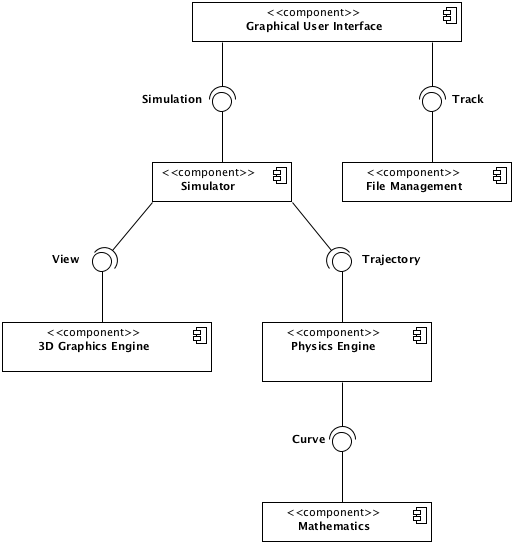
\includegraphics[width=\linewidth]{bilder/component_overview}
\caption{Komponentendiagramm für den Achterbahnsimulator}
\label{labelname}
\end{figure}

\section{Schnittstellenspezifikation}

Im Folgenden werden die einzelnen Schnittstellen der Komponenten aus der
Komponentenspezifikation näher erläutert, d. h. die von ihnen zur Verfügung
gestellten Operationen werden dokumentiert. Die Tabelle ist dabei um so viele
Zeilen zu erweitern, wie es Schnittstellen im Komponentendiagramm gibt. In der
innen liegenden Aufteilung ist für jede Operation einer Schnittstelle eine
Zeile einzufügen.  Reine Set- und Get-Aufrufe brauchen nicht aufgeführt zu
werden (sollten auch möglichst nicht komponentenübergreifend auftauchen).

\begin{tabular}[ht]{|l|p{0.35\linewidth}|p{0.35\linewidth}|}
 \hline
 Schnittstelle & \multicolumn{2}{|c|}{Aufgabenbeschreibung}\\
 \hline
 \hline
    /S10/ Track & \multicolumn{2}{|c|}{Spezifikation der Achterbahn mit Stützstellen und Parametern}\\
 \hline
 & getCurve() : Curve & Liefert die Achterbahnstrecke als mathematische Raumkurve zurück.\\ 
 \hline
    /S20/ Curve & \multicolumn{2}{|c|}{Repräsentation einer ortientierten Raumkurve}\\
 \hline
 & getLength() : double & Liefert die Länge der Raumkurve.\\ 
 & getPoint(lengh : double) : CurvePoint & Liefert den Repräsentanten für einen bestimmen Punkt auf der Raumkurve zurück,
 wobei über die Bogenlänge parametrisiert wird.\\ 
 & getPointSequence(maxDistance : double, maxAngle : double) : List<CurvePoint> &
 	Liefert eine Liste mit Punkten auf der Raumkurve wieder, die höchsten den angegebenen Abstand und die
 	Differenz im Raumwinkel haben dürfen. \\
 \hline
    /S21/ CurvePoint & \multicolumn{2}{|c|}{Repräsentation eines bestimmten Punktes auf einer Raumkurve}\\
 \hline
 & getPosition() : Vector & Liefert die Position. \\
 & getRollAxis() : Vector & Liefert die Rollachse (Längsachse).\\ 
 & getPitchAxis() : Vector & Liefert die Nickachse (Querachse). \\ 
 & getYawAxis() : Vector & Liefert die Gierachse (Hochachse). \\
 \hline
 	/S30/ Trajectory & \multicolumn{2}{|c|}{Bahnkurve einer Punktmasse als Funktion der Zeit}\\
 \hline
 & getCurve() : Curve & Liefert den räumlichen Verlauf der Bahnkurve als Raumkurve zurück.\\ 
 & getPoint(time : double) : TrajectoryPoint & Liefert den Repräsentanten für einen bestimmten Punkt auf der Bahnkurve zurück.\\ 
 %& Name der Funktion3 & Beschreibung3\\ 
 %& Name der Funktion4 & Beschreibung4\\ 
 \hline
 	/S31/ TrajectoryPoint & \multicolumn{2}{|c|}{Repräsentation eines bestimmten Punktes auf der Bahnkurve}\\
 \hline
 & getPosition() : Vector & Liefert die momentane Position.\\ 
 & getVelocity() : Vector & Liefert die m. Geschwindigkeit.\\ 
 & getAcceleration() : Vector & Liefert die m. Beschleunigung. \\ 
 \hline
 \end{tabular}

\begin{tabular}[ht]{|l|p{0.35\linewidth}|p{0.35\linewidth}|}
 \hline
 Schnittstelle & \multicolumn{2}{|c|}{Aufgabenbeschreibung}\\
 \hline
 \hline
    /S40/ Simulation & \multicolumn{2}{|c|}{Repräsentant für eine konkrete Simulation}\\
 \hline
 & start() : void & Startet die Simulation.\\ 
 & stop() : void & Stoppt die Simulation. \\ 
\hline
	/S50/ View & \multicolumn{2}{|c|}{Repräsentant für die 3D-Welt mit bestimmter Kameraperspektive}\\
\hline
 & setCamera(positon : Vector, direction : Vector) & Setzt die Kamera auf die angegebene Position und Raumrichtung. \\ 
 \hline

 & setCurve(curve : Curve) & Setzt die Bahndaten die zur Darstellung kommen sollen. \\ 
 \hline

 \end{tabular}





\section{Protokolle für die Benutzung der Komponenten}

%In diesem Abschnitt wird mit Hilfe von Protokoll-Statecharts die korrekte
%Verwendung der zu entwickelnden Komponenten dokumentiert. Dies ist insbesondere
%für diejenigen Komponenten notwendig, für die eine Wiederverwendung möglich
%erscheint oder sogar bereits geplant ist.

%Begründen Sie für welche Komponenten eine Wiederverwendung sinnvoll erscheint
%und für welche nicht!
Der Achterbahnsimulator setzt trotz seines (schon durch den Namen ersichtlichen)
eingeschränkten Anwendungsbereiches bereits alle wesentlichen Teile für die
Simulation anderer mechanischer Systeme um: die Berechnung der Bewegung von
Punktmassen wird auch ohne Einschränkung auf konkrete Kurven abgedeckt. Es liegt
deswegen nahe, diese Komponente sauber zu kapseln und wiederverwendbar zu gestalten.

Die Benutzeroberfläche ist eine konkret auf die Funktionalität der Anwendung
zugeschnittene Komponente. Allerdings dürfte die Oberfläche ohne größere
Schwierigkeiten auf andere Simulatoren neben Achterbahnen verallgemeinerbar sein.
Jede andere Art von Anwendung dürfte einen anderen Satz an Dialogfenstern und
Menübefehlen benötigen und andere Informationen auf dem Bildschirm darstellen,
so dass bei dieser Komponente ingesamt kein größerer Aufwand für eine
Wiederverwertung aufgebracht werden sollte.

Die 3D-Anzeige ist ebenfalls nicht auf bestimmte Modelle eingeschränkt, zumal in
der geplanten Architektur alle Dekorationen dynamisch zugefügt werden können.
Allerdings ist das zum Einsatz kommende 3D-Framework selber schon von sich aus 
für die Wiederverwertung ausgelegt, so dass der Mehrwert der eigenen Komponente
zumindest angezweifelt werden. Erst im Zusammenspiel mit dem Simulator und der 
Benutzeroberfläche erscheint der Mehraufwand für eine allgemeinere Schnittstelle
vertretbar.

Die Dateiverwaltung ist eine auf das Einlesen der vorgegebenen XML-Spezifikation 
zugeschnittene Spezialkomponente. Schon bei Änderung des Dateiformates wäre eine
umfangreiche Änderung angebracht. Eine Wiederverwertbarkeit scheint ausgeschlossen.

Alle mathematischen Routinen sollten selbstverständlich möglichst allgemein und
wiederverwertbar entworfen werden. Es muss nur sichergestellt werden, dass die
Implementierungen effizient bleiben.
